\documentclass{tufte-handout}

%\geometry{showframe}% for debugging purposes -- displays the margins

\usepackage{amsmath}


% Set up the images/graphics package
\usepackage{graphicx}
\setkeys{Gin}{width=\linewidth,totalheight=\textheight,keepaspectratio}
\graphicspath{{graphics/}}


% The following package makes prettier tables.  We're all about the bling!
\usepackage{booktabs}

% The units package provides nice, non-stacked fractions and better spacing
% for units.
\usepackage{units}

% The fancyvrb package lets us customize the formatting of verbatim
% environments.  We use a slightly smaller font.
\usepackage{fancyvrb}
\fvset{fontsize=\normalsize}

% Small sections of multiple columns
\usepackage{multicol}

% Provides paragraphs of dummy text
\usepackage{lipsum}

% These commands are used to pretty-print LaTeX commands
\newcommand{\doccmd}[1]{\texttt{\textbackslash#1}}% command name -- adds backslash automatically
\newcommand{\docopt}[1]{\ensuremath{\langle}\textrm{\textit{#1}}\ensuremath{\rangle}}% optional command argument
\newcommand{\docarg}[1]{\textrm{\textit{#1}}}% (required) command argument
\newenvironment{docspec}{\begin{quote}\noindent}{\end{quote}}% command specification environment
\newcommand{\docenv}[1]{\textsf{#1}}% environment name
\newcommand{\docpkg}[1]{\texttt{#1}}% package name
\newcommand{\doccls}[1]{\texttt{#1}}% document class name
\newcommand{\docclsopt}[1]{\texttt{#1}}% document class option name


%%% Additions to template by DSL
\usepackage{hyperref} % provides \url{}
% remove separation between list items http://tex.stackexchange.com/a/10689/1783
\usepackage{enumitem}
\setlist{nosep}


\title{Implementing the Teachings of Edward Tufte}
\author{Kristy Wendt}
\date{16 June 2015}  % if the \date{} command is left out, the current date will be used
\begin{document}

\maketitle% this prints the handout title, author, and date


\begin{abstract}
\noindent \textsc{Handouts should be made to complement serious presentations.} 
The purpose of this handout is to summarize the Edward Tufte lecture on June 16th, 2016 in Chicago.  

Tufte began and ended his lecture wordlessly with a clip from the Music Animation Machine project and it is one of the metaphors used for the beautiful potential of  clarity in information display.  Relatively large amounts of information are displayed in context; the data contains the past, present, and future, and in a short matter of time, the viewer can predict the duration, pitch and sound of the notes heard based on the visual experience of the data.  This is a beautiful metaphor for the potential of immediate visual context in multiscale imaging.
\end{abstract}




\marginnote[-5cm]{
\textsc{Agenda:}
\begin{description}
\item{1} Beautiful Data
\item{2} Thoughtful Web Content  
\item{3} Every Meeting Begins with a Document
\item{4} Evidence Decays, but Analytical Thinking is Forever 
\item{5} Presentation 
\item{6} Spectatorship  
\item{7} Final Comments
\end{description}
}

\begin{marginfigure}
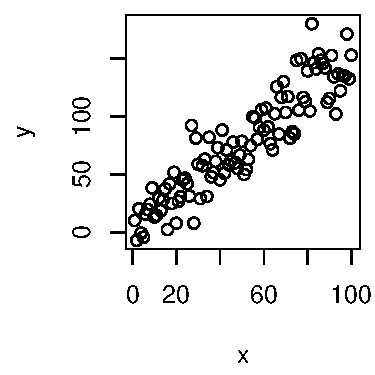
\includegraphics{Figure1}
\caption{Beautiful data is adjacent in space, not stacked in time. See Music Animation Machine: https://www.youtube.com/watch?v=OxM--mALGXc}
\end{marginfigure}








\section{Thoughtful Web Content}



\subsection{Deconstructing Success in the Wilderness}



\newthought{Play in the Big Leagues} in the presentation of your web content.  That is, reference the sources that Tufte calls "successful in the wild:"  Tufte pulls up a story from the \textit{New York Times} and deconstructs the content display.  For little data, no data graphics, clear icons, and information is adjacent in space, not stacked in time.  At the bottom of the \textit{New York Times} site is a list that Tufte notes, "appeals to every possible constituency" (Figure 2).  



\begin{marginfigure}
\includegraphics{Figure2}
\caption{At the bottom of the \textit{New York Times} is a list that Tufte notes, appeals to "every possible constituency."}
\end{marginfigure}



Always put your name on your work. Don't say "we" in presentations.

Sentences have agency. They are powerful for thinking. Stop using bullet points.

Whenever possible, get the story out of your voice and into the voice of authority.

Little data is always numbers in sentences (Figure 3).

If in doubt, pull up a \textit{New York Times} piece, or an \textit{ESPN} report and put it alongside your content. In N\textit{ew York Times} graphics, the emphasis is on the highs and lows of the data, rather than x and y axis.  Data is always in contextual order, never alphabetical order.


\section{Every Meeting Begins with a Document}



\begin{marginfigure}
\includegraphics{Figure3}
\caption{A clip from the \textit{New York Times} showing "little data" as numbers in sentences.}
\end{marginfigure}

\newthought{20\% shorter meetings occur naturally} when you put your content adjacent in space, rather than stacked in time, and no one complains.  Tufte recommends using an 11 X 17" paper -- filling it with the information normally contained in 50-100 PowerPoint slides -- and folding it in half, but we can use this template that I have modified from LaTex to accomplish similar goals.  It may seem time/labor intensive, but I can help.  When you document your presentation this way, every move is about content, and you accommodate everyone's cognitive style. What is important is high on the page. During a meeting, take notes when someone asks a question. Never embarrass a questioner. No meeting should exceed 24 minutes.


\begin{marginfigure}
\includegraphics{Figure4}
\caption{"Why Most Published Research Findings are False," a controversial and highly cited article by John Ioannidis.}
\end{marginfigure}




\section{Evidence Decays, but Analytical Thinking is Forever}


\subsection{Every Move is About Content}



\newthought{The only constant is change.} Tufte cites "Why Most Published Research is False" Ioannidis, \textit{PLOS} (Figure 4).  There is an evidence decay cycle, and only around 1\% of content ever ends up being cited. Tufte notes, "You may have a stalker, or an Assistant Professor may be citing your work for a grant, but in both cases, they are only reading your abstract.  So really work on that abstract.  It should clearly state what the problem is, who cares, and what you're going to do about it.  Stated again: problem, relevance, solution.  Work on your abstract early.  


\begin{marginfigure}
\includegraphics{Figure6}
\caption{Maps show information with differentiated lines all the time with greater richness than art history charts and network drawings.  Cartographic lines have a high-resolution and lightness and clarity, similar to typography}
\end{marginfigure}


Similarly, imbue your data with longevity by focusing on 1) causality, 2) comparison (3 or 4 variables) and 3) mechanism.  Look in Overleaf for LaTex (what I used to make this handout )for table templates used in \textit{Nature}.  In your presentation of data, be driven not by process, but by content.  Always pre-specify your methods of display.  Put information in your linking lines. Shift from pronouns to what things do. 



Refer to Figure 5.  The SARS graphic focuses on causality, has multiple sources and levels of data, annotated linking lines, annotated nouns (patient names with virus strain identification) and efficiency of design and credibility.  Google "Links, Causal Arrows, and Networks" to view on Tufte site.


\begin{marginfigure}
\includegraphics{Figure5}
\caption{This practical, workaday diagram demonstrates good analytical practices in displays that use links to and arrows to tie together nouns, displays such as process, historical narratives, trees, networks, organization charts, project management charts, and the like.}
\end{marginfigure}


In data displays, use the most widely used graphic in human history as your metaphor - Google maps (Figure 7).  In a map, the color has gray value, information is spread in space rather than stacked in time, information is not aggressively segregated from the user. There is no operating system. Nothing is segregated by mode of production. See Figure 8, next page. Use a natural color palate.




\begin{marginfigure}
\includegraphics{Figure7}
\caption{The metaphor is the map.}
\end{marginfigure}


\section{Presentation}

\subsection{Know Your Content, Respect your Audience}


\begin{marginfigure}
\includegraphics{Figure11}
\caption{Wach the Viz-O-Matic video by Wayne Lytle. https://youtu.be/fP-7rhb-qMg}
\end{marginfigure}

\newthought{The rules for presentation in academic pursuits are parallel to spectatorship} and the two skills complement one another.  In your presentations, always provide downlinks to material.  

The three dangers within your academic community are 1) stupidity, 2) conspiracy, and 3) malice and in most cases the problem is stupidity.  Be as hard-headed about identifying stupidity in content as you would be in hiring a new employee. 


Your motives are no better or worse than any of your colleagues.



Do not fear negative feedback.  In the evolution of \textit{homo sapiens}, disproportionate weight on negative feedback was necessary for survival; we needed to act fast to potential threats. Too often, we tend to disproportionately react to negative feedback and criticism.  Take a breath.  


Remember, there are evil people in the world, but they are probably not your colleagues.  Take questions, but never condescend to the questioner. Keep in mind most questions arise from personal concerns.


\marginnote[-5cm]{
\textsc{Your motives are no better or worse than any of your colleagues. -Edward Tufte}

}


Do not be stupid.  Demonstrate mastery of detail in your presentations.  Do not throw jargon in the air. Do not fly so high in the air.  We are all reasoning analytically.  Your presentations should demonstrate a hands-on quality.  Not personal, not first-person, Follow PGP: particular/general/particular when presenting complicated material. Take the broad view, but don't forget to dive in and demonstrate your mastery of some relevant detail of the content.

Know your content. In marketing, too much emphasis is placed on knowing your audience, but great companies don't do a lot of market research.  Know your content, and respect your audience.  Give your audience endless respect.  Think the best you possibly can of your audience.  You are lucky to be there. Isn't this great?

Practice intensely beforehand.

Do not pander.  Tufte mentions watching some of the best online courses at MIT, and watching professors pander to the students.  "How was everybody's weekend?" Don't do it.
% * <kwendt3@wisc.edu> 2015-06-24T14:49:46.296Z:
%
% 
%
% * <kwendt3@wisc.edu> 2015-06-24T14:49:44.778Z:
%
% 
%

Express enthusiasm, but only if your enthusiasm is real.

Use humor only if it is relevant to your content.

Finish early.


\section{Spectatorship}
\subsection{See with an Open Mind, not an Empty Head}
Stay on the content.  That's why you are there.


\begin{marginfigure}
\includegraphics{Figure8}
\caption{An open mind does not mean an empty head.}
\end{marginfigure}

See with an open mind, but not an empty head (Figure 9).  Give your undivided attention as long as you can. Loot. Don't let a contrary thought spoil the seeing, maybe you'll learn something.  Sit at the back.  After 2 or 3 absurdities, walk. Don't go meta. Don't be prematurely judgmental. Listen, see, think, learn. 

When you present, you want people to think.

Practice data thinking.  Use your best cognitive sense: what is relevant? How important is it?  What problems will we work on? Learn the art of the solvable problem.

\section{Final Comments}

Analytical thinking is forever.

Annotate everything. If in doubt, use small multiples. 


\begin{marginfigure}
\includegraphics{Figure10}
\caption{The classic severe storm animation from Tufte's Visual Explanations. This image was created in a collaboration between Tufte and the University of Illinois National Center for Supercomputing Applications. Posted by permission Edward R. Tufte, Visual Explanations, Graphics Press, Cheshire, CT, 1997.}
\end{marginfigure}


Small multiples are a visualization concept introduced by Edward Tufte. Tufte spent some time showing Image Quilt, which uses google search to create small multiple images. 

Small multiples are:

"Illustrations of postage-stamp size are indexed by category or a label, sequenced over time like the frames of a movie, or ordered by a quantitative variable not used in the single image itself."

In other words, small multiples use the same basic graphic or chart to display difference slices of a data set. Small multiples can show rich, multi-dimensional data without trying to cram all that information into a single, overly-complex chart. Small multiples go by many names, including Trellis Chart, Lattice Chart, Grid Chart, and Panel Chart. I would even argue that sparklines are a simpler, smaller cousin of small multiples.

What problem does this solve?

Small multiples offer a few valuable features:

They allow for the display of many variables with less risk of confusing your audience. Trying to display three or more variables in a single chart is a challenge Stephen Few calls overplotting (PDF).
The reader can quickly learn to read an individual chart and apply this knowledge as they scan the rest of the charts. This shifts the reader's effort from understanding how the chart works to what the data says. That's a worthy goal in all data presentation.

Small multiples enable comparison across variables and reveal the range of potential patterns in the charts.



\begin{marginfigure}
\includegraphics{Image11}
\caption{An image quilt of a Feynman Diagram by Adam Schwartz.}
\end{marginfigure}





\vspace{1cm}



\vspace{1cm}


\end{document}
